\subsubsection{Cơ sở hạ tầng dưới dạng mã (Infrastructure as Code - Terraform)}

Trong kỹ thuật phần mềm,
việc cấu hình
cơ sở hạ tầng theo phương pháp thủ công
thường tiềm ẩn nhiều rủi ro
gây sai sót, tốn thời gian
và gặp khó khăn trong việc tái khởi tạo một cách chính xác.
Ngoài ra, việc dọn dẹp hoặc hủy bỏ tài nguyên thủ công dễ dẫn đến tình trạng sót tài nguyên, gây lãng phí và rủi ro bảo mật.
Việc sử dụng Infrastructure as Code (IaC) sẽ khắc phục được vấn đề đó.

\begin{block}{Ứng dụng trong đồ án}
Trong phạm vi đồ án này,
em sử dụng Terraform
để quản lý cấu hình một số hạ tầng của các nhà cung cấp
có hỗ trợ terraform giúp định nghĩa
và quản lý hạ tầng của dự án một cách tự động thay
vì thao tác thủ công.

\end{block}

Tại repo infra-by-terraform
dùng root module lớn truyền biến
vào các module nằm trong thư mục modules.
Tuy nhiên việc chạy CI/CD có thể xảy ra lỗi vì provider bị lỗi,
hoặc mất thời gian
khi hệ thống bắt buộc phải thực hiện
lệnh \texttt{terraform init} cho toàn bộ các \textit{provider}
mặc dù chỉ có một thay đổi nhỏ ở một dịch vụ cụ thể.
Vì vậy, trong đồ án này,
em sử dụng mỗi provider trong folder riêng tại repo
infrastructure.
Kết hợp github action chỉ
kích hoạt quy trình kiểm tra
và triển khai Terraform khi và chỉ khi có
sự thay đổi dữ liệu bên trong thư mục của \textit{provider} tương ứng.

\begin{figure}[H]
\centering
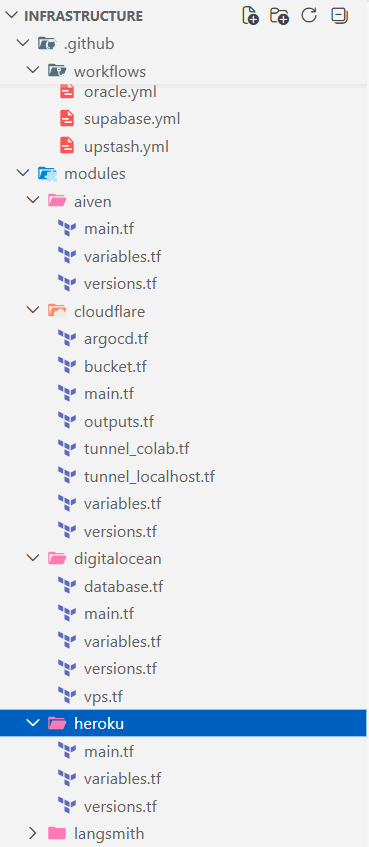
\includegraphics[width=0.45\textwidth]{pictures/infrastructure-project-v2.png}
\caption{Cấu trúc thư mục dự án Terraform theo từng Provider}
\end{figure}

Hạ tầng của hệ thống quản lý qua các dịch vụ bao gồm:

\begin{itemize}
\item \textbf{Oracle Cloud Infrastructure (OCI):} Khởi tạo và quản lý máy chủ ảo (VPS) phục vụ triển khai ứng dụng.
\item \textbf{Aiven:} Khởi tạo Kafka trung chuyển tin nhắn hệ thống.
\item \textbf{Supabase:} Cấu hình cho dịch vụ xác thực người dùng (Auth Service).
\item \textbf{LangSmith:} Quản lý các tài nguyên phục vụ giám sát và đánh giá chuỗi RAG (LangChain, LangGraph).
\item \textbf{Cloudflare:} Quản lý cấu hình DNS, lưu trữ đối tượng (Cloudflare R2 Bucket) và thiết lập các đường truyền an toàn (Cloudflare Tunnel).
\item \textbf{Neon:} Khởi tạo và quản lý các CSDL PostgreSQL độc lập cho từng vi dịch vụ (Microservices).
\item \textbf{DigitalOcean:} Cấu hình CSDL PostgreSQL phục vụ riêng cho luồng thu thập dữ liệu (Data Pipeline VBPL).
\item \textbf{Heroku:} Triển khai và quản lý môi trường cho dịch vụ thanh toán (Payment Service).
\end{itemize}

\begin{figure}[H]
\centering
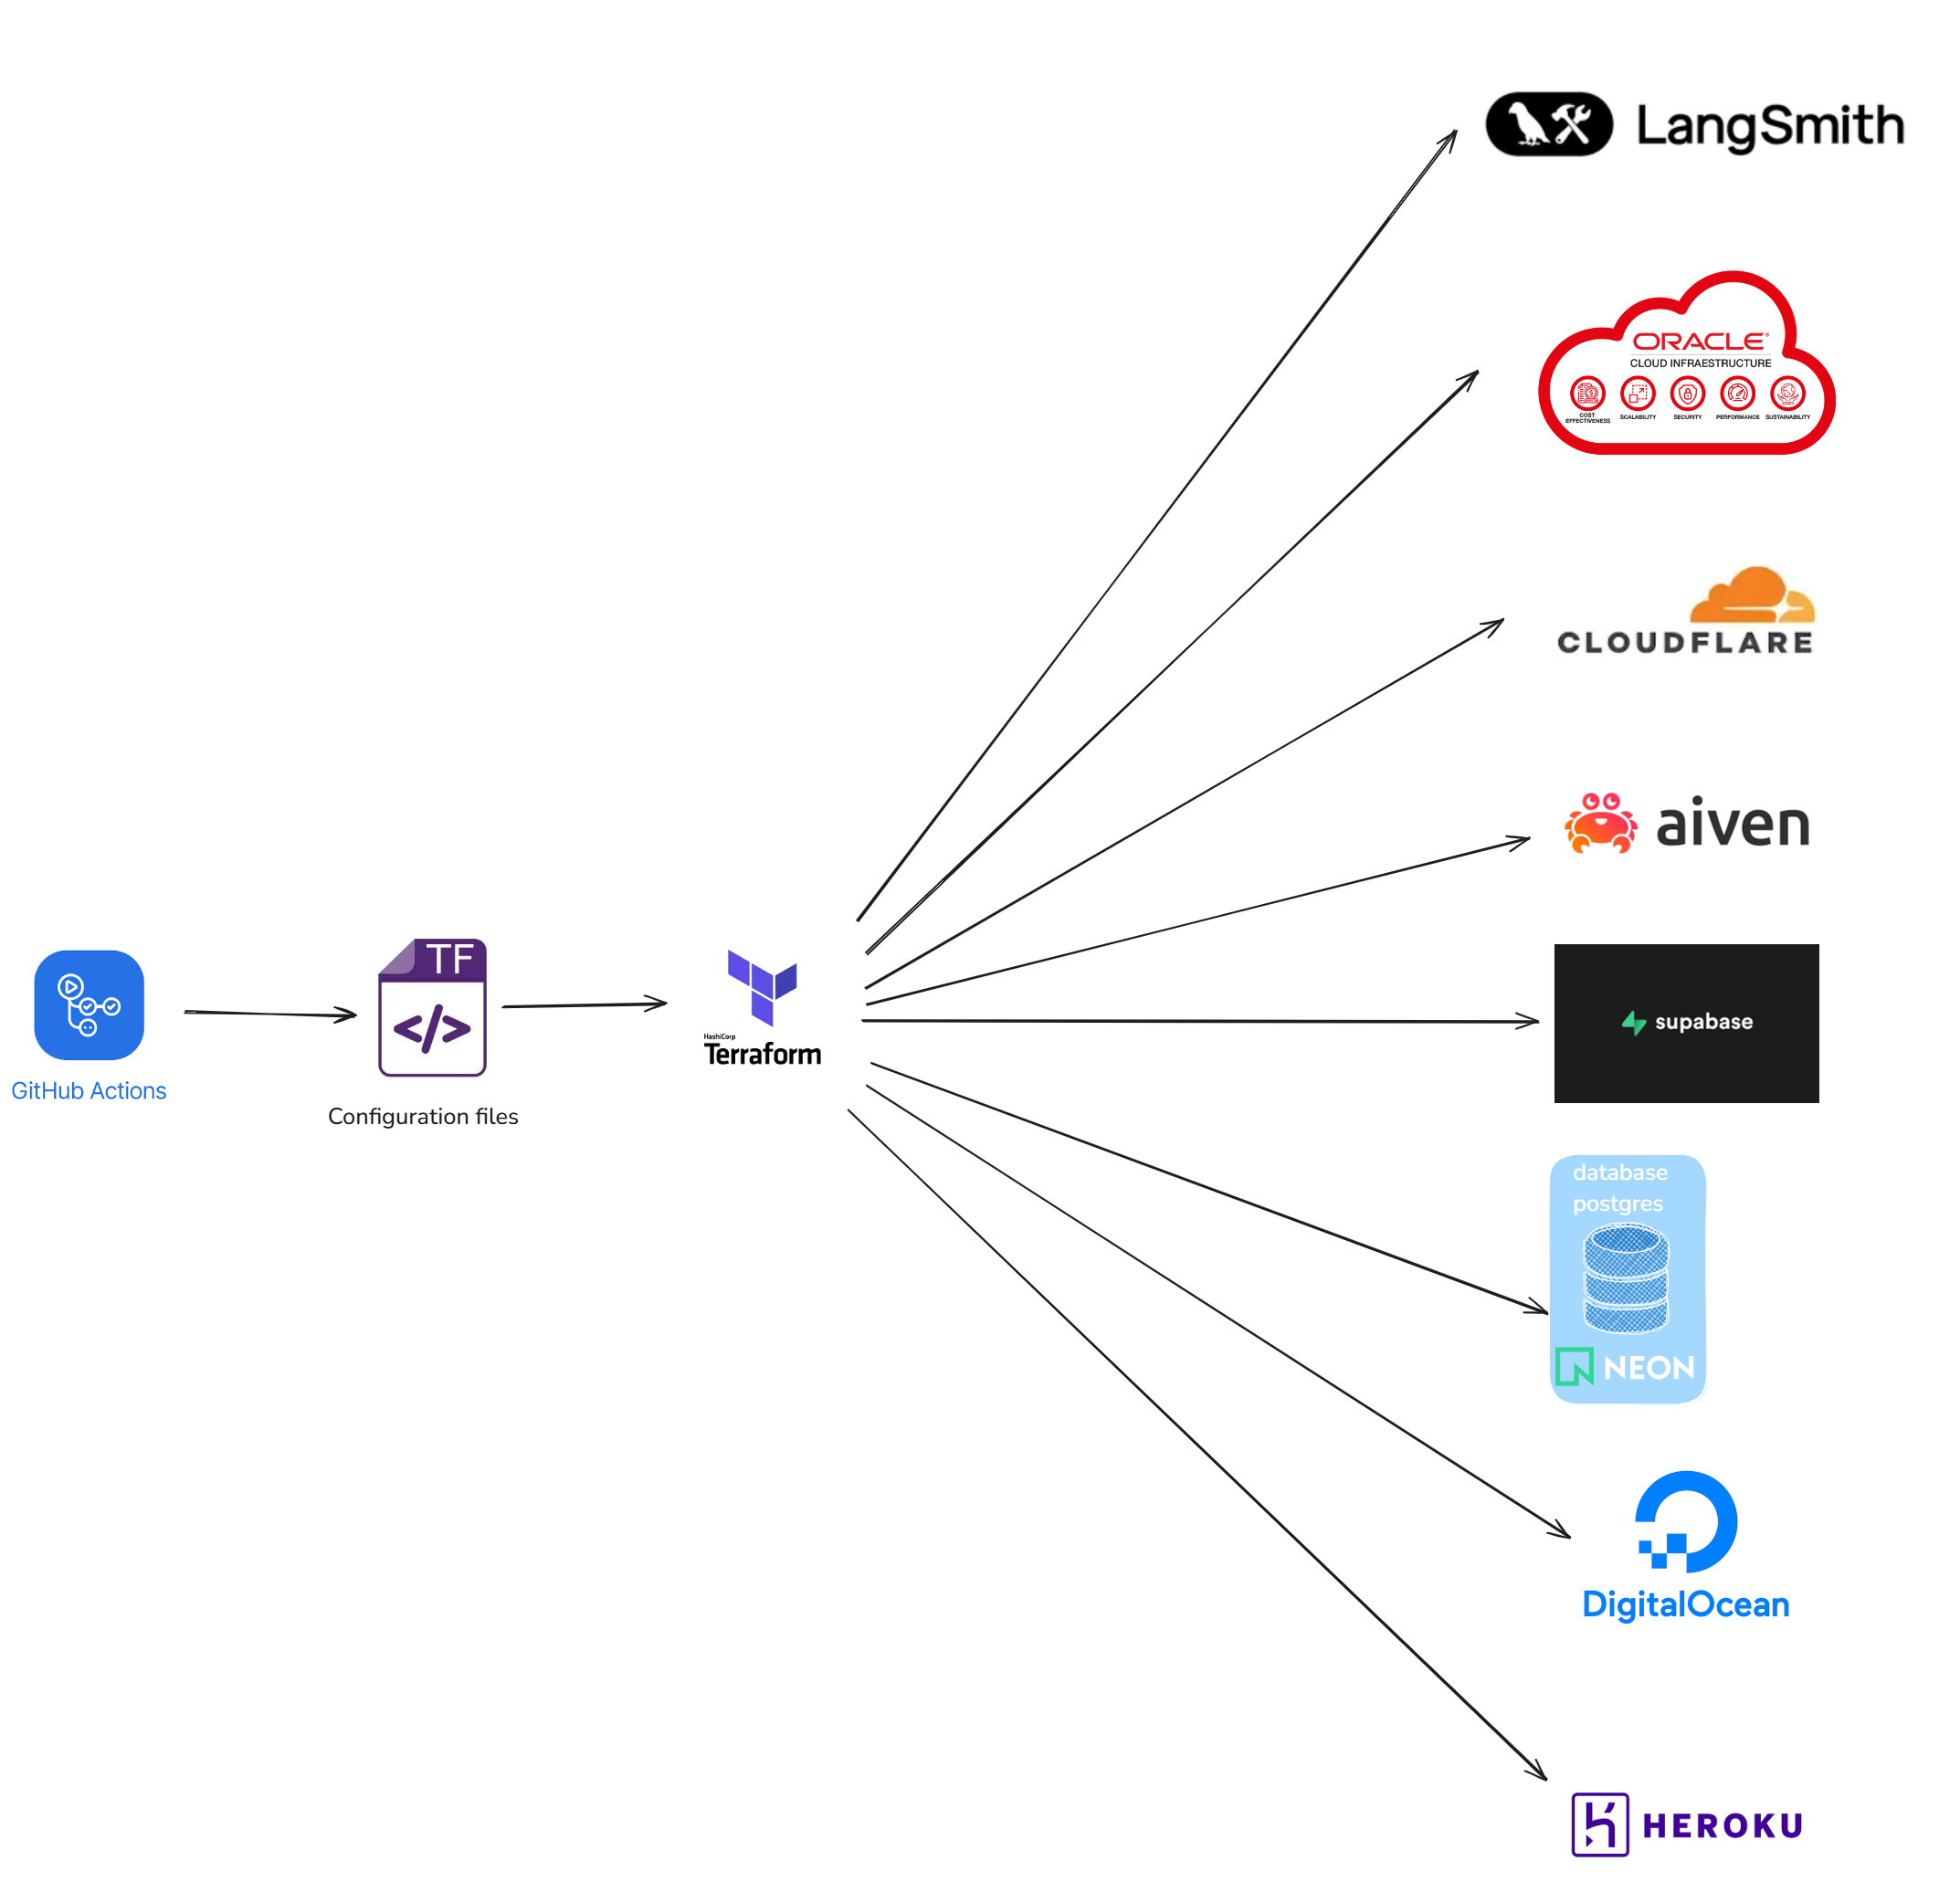
\includegraphics[width=0.5\textwidth]{pictures/infrastructure-as-code-IaC-terraform.excalidraw.png}
\caption{Sơ đồ tổng quan quản lý hạ tầng bằng Terraform trong dự án}
\end{figure}

Bên cạnh đó, dự án sử dụng giải pháp
Terraform Cloud đóng vai trò làm \textit{Remote Backend}
để lưu trữ trạng thái (\textit{State File}).
% tập trung và an toàn,

\begin{figure}[H]
\centering
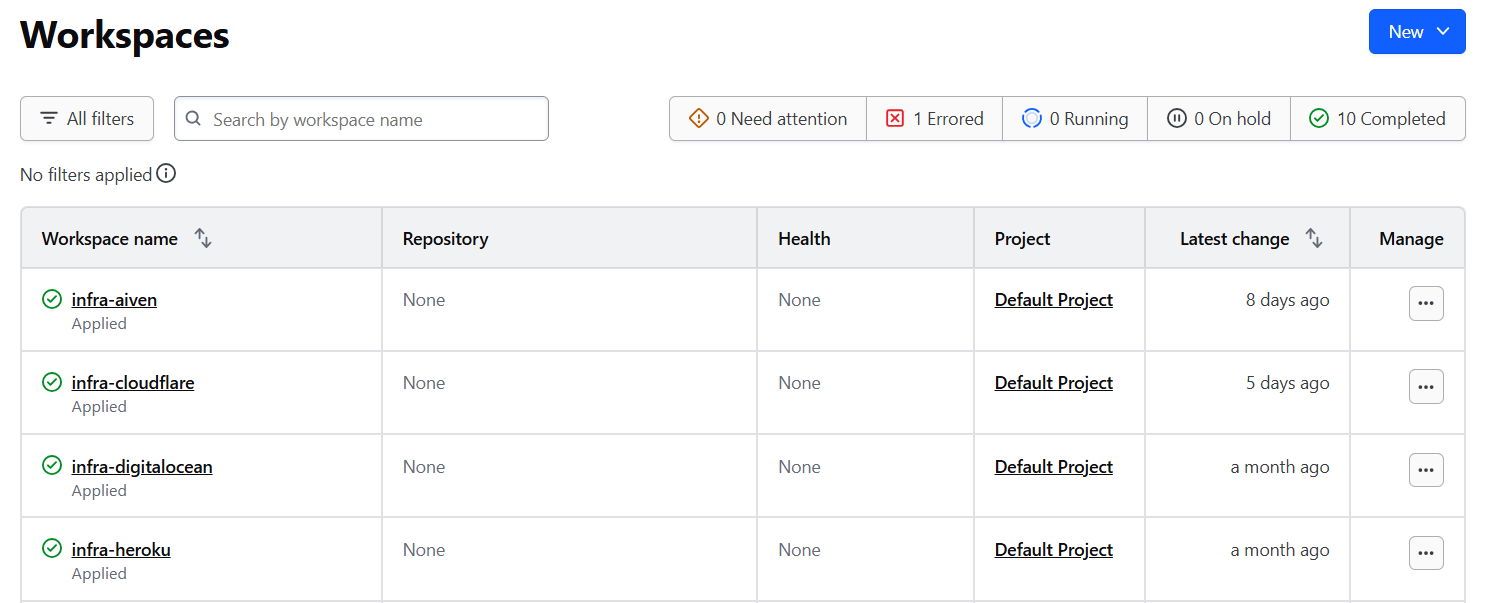
\includegraphics[width=0.95\textwidth]{pictures/terraform-hub-web-ui.png}
\caption{Giao diện quản lý trạng thái tập trung trên Terraform Cloud}
\end{figure}

Dưới đây là một vài kết quả
các tài nguyên được khởi tạo tự động
thông qua mã nguồn Terraform thành công:

\begin{figure}[H]
\centering
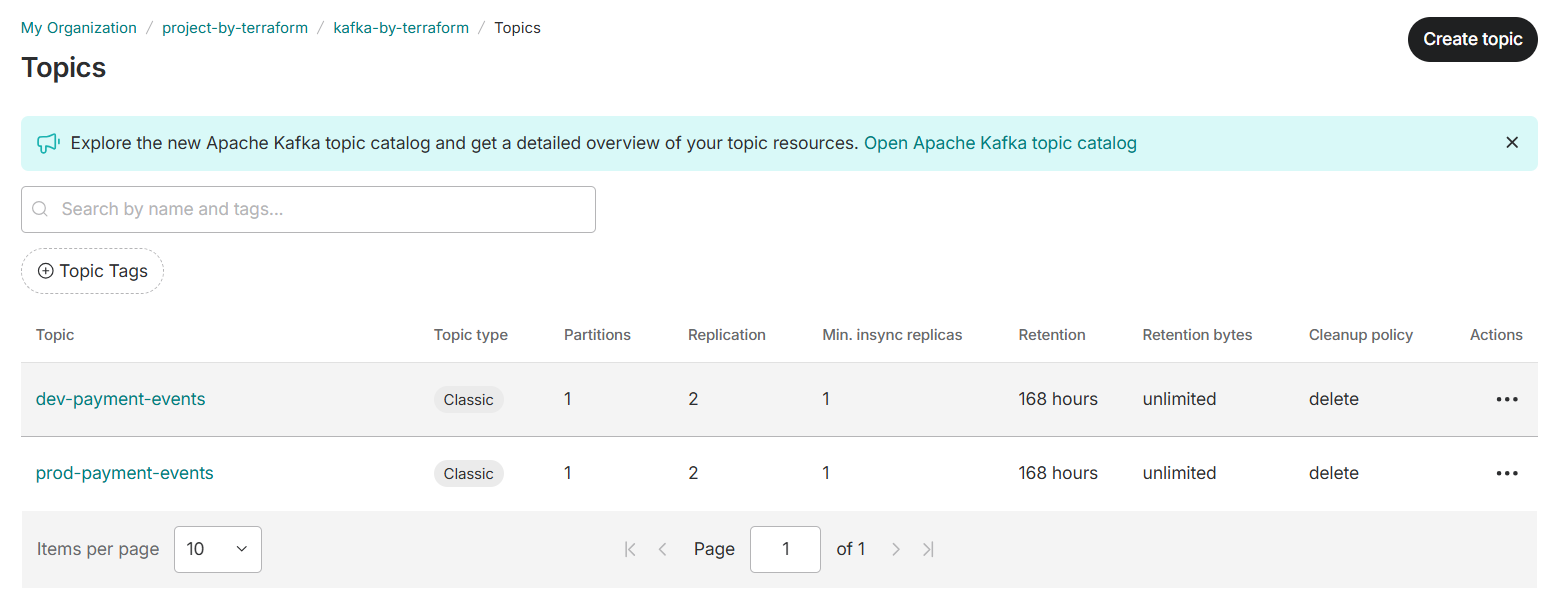
\includegraphics[width=0.95\textwidth]{pictures/kafka-aiven-terraform.png}
\caption{Dịch vụ Kafka trên nền tảng Aiven được cấu hình tự động}
\end{figure}

\begin{figure}[H]
\centering
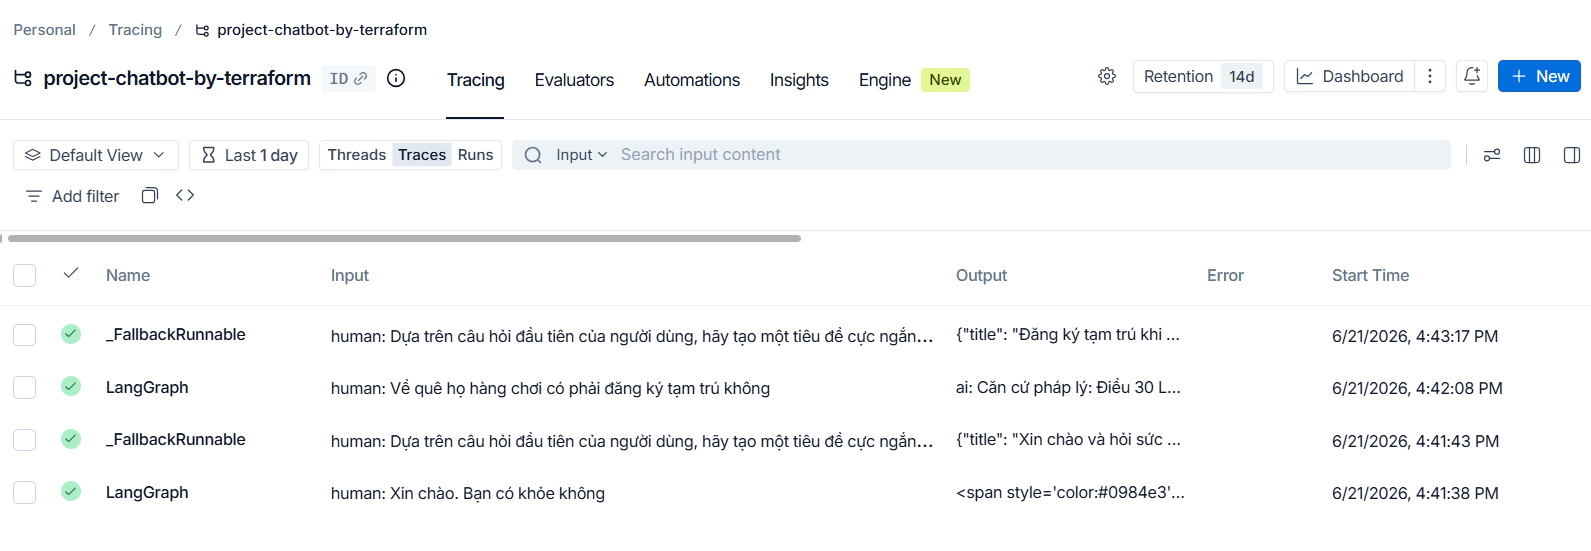
\includegraphics[width=0.95\textwidth]{pictures/langsmith-terraform.png}
\caption{Dự án LangSmith được tạo từ terraform cho dịch vụ chatbot}
\end{figure}

\begin{figure}[H]
\centering
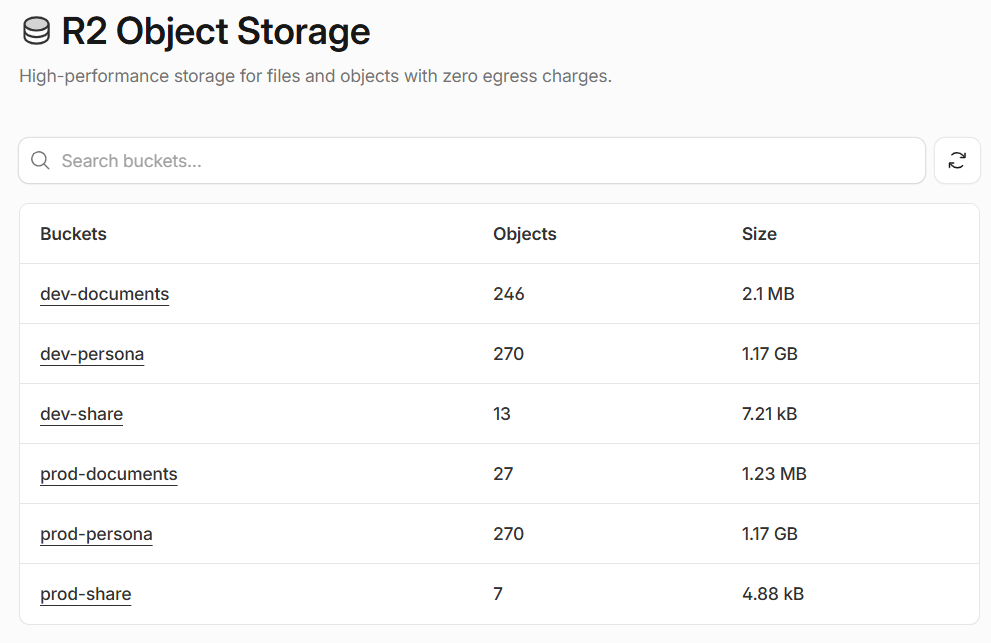
\includegraphics[width=0.95\textwidth]{pictures/cloudflare-r2-terraform.png}
\caption{Cấu hình các R2 Bucket thành công trên Cloudflare}
\end{figure}

Do chính sách tài khoản miễn phí của Neon có nhiều giới hạn về tài nguyên,
trong mã nguồn Terraform,
em đã cấu hình tách biệt hoàn toàn thành các dự án riêng lẻ trên Neon
cho từng môi trường và dịch vụ.
Từ đó, đảm bảo sự độc lập dữ liệu và tránh giới hạn
miễn phí.
% nhằm tối ưu hạn mức và đảm bảo tính độc lập dữ liệu.

\begin{figure}[H]
\centering
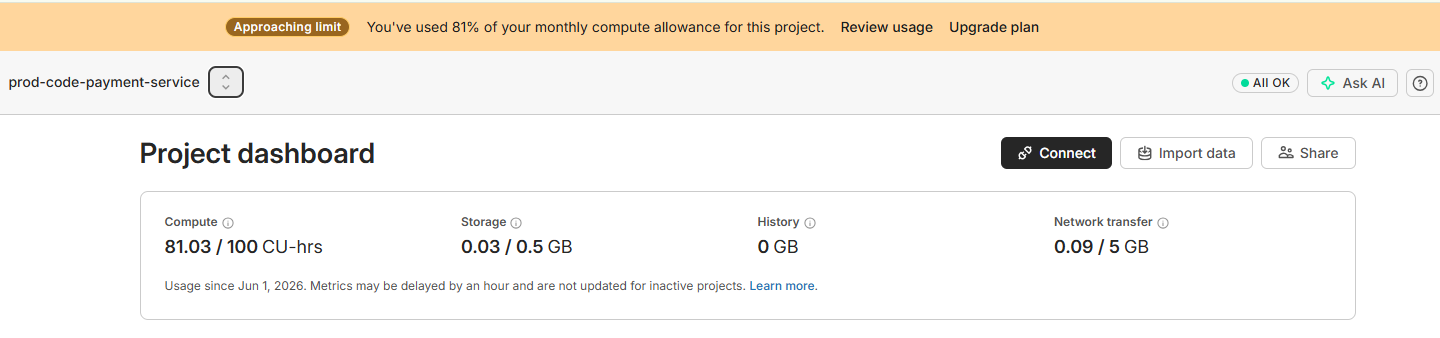
\includegraphics[width=0.95\textwidth]{pictures/neon-limit-free.png}
\caption{Thông báo giới hạn tài nguyên của tài khoản miễn phí trên Neon}
\end{figure}
